\documentclass[10pt,a4paper]{book}
        
\usepackage{amssymb}% for numbers/numbers
\usepackage{lscape}

\usepackage{sectsty}
\allsectionsfont{\sffamily}

\setlength{\textheight}{24cm}
\setlength{\textwidth}{15.912cm}

\setlength{\evensidemargin}{0cm}
\setlength{\oddsidemargin}{0cm}

\setlength{\topmargin}{-0.5cm}
%\setlength{\parindent}{0cm}


\usepackage{listings}
\usepackage{color}
\lstdefinestyle{defaultstyle}{}
\lstset{language=Python}
\lstset{basicstyle=\ttfamily}
\lstset{showstringspaces=fales}
\lstset{keywordstyle=\color{blue}}
\lstset{frame=single}
%\lstset{backgroundcolor=\color{white},emph={EMPTY},emphstyle=\color{white}}
%\definecolor{lightgrey}{cmyk}{0.1,0.1,0.1,0}
%\lstset{backgroundcolor=\color{lightgrey}}

\renewcommand{\labelitemii}{\ensuremath{\triangleright}}    %  open triangle replaces default dash

\newcommand{\py}[1]{\texttt{\color{blue}#1}}

\newcommand{\nmesh}{nmesh}

\usepackage{graphicx}

\usepackage[dvips=true,bookmarks=true]{hyperref} 


\begin{document} 



\title{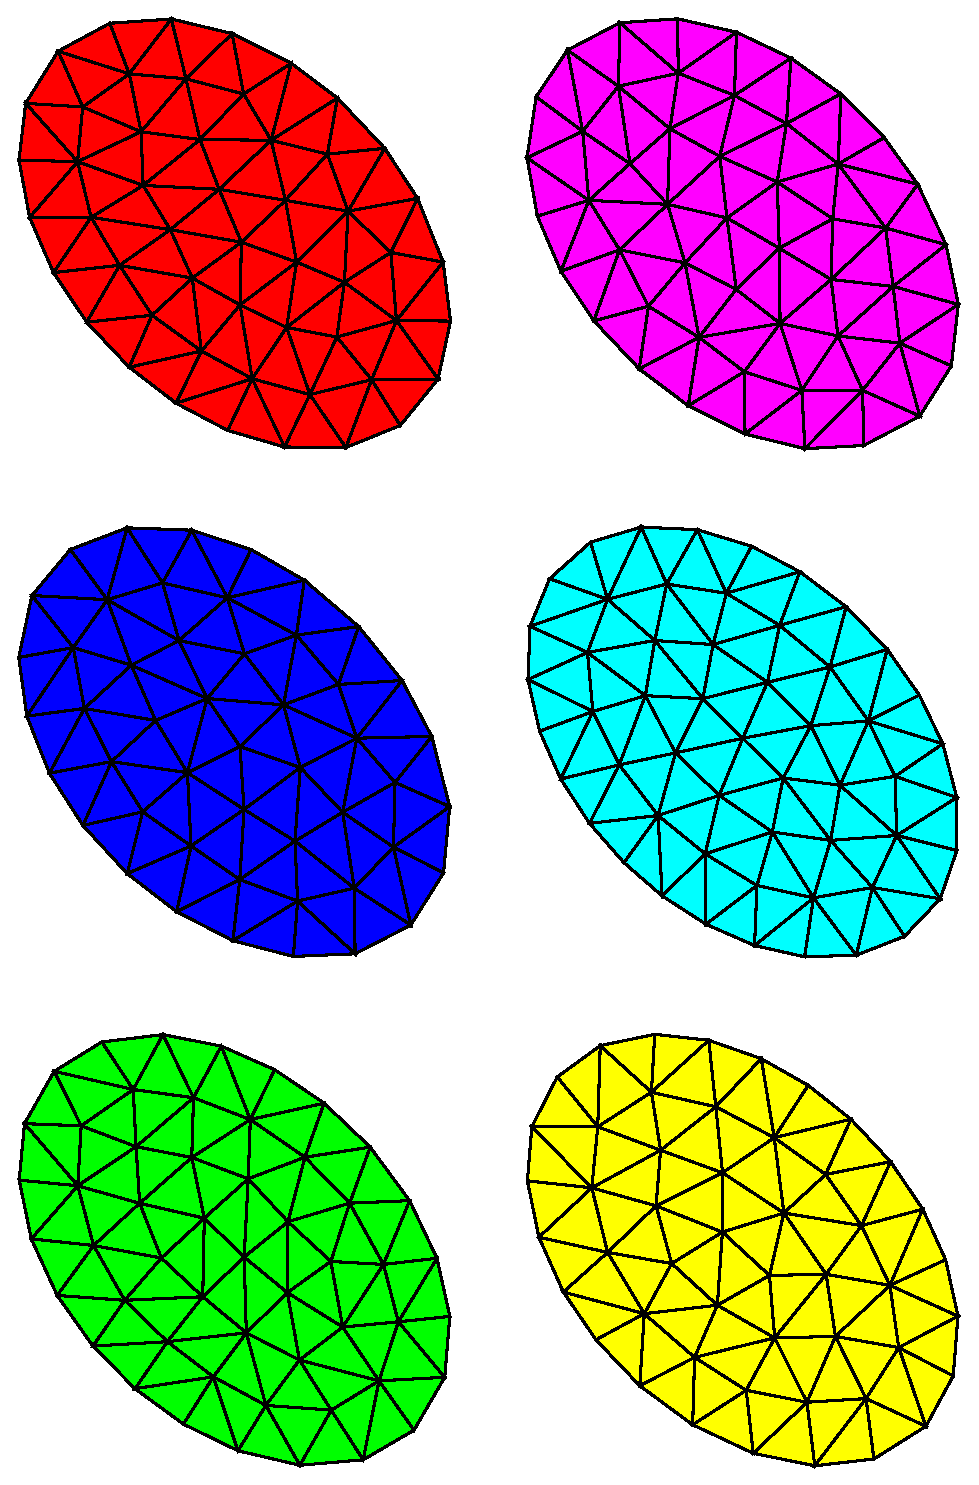
\includegraphics[width=5cm]{plots/somemesh}\\[2cm] 
\sffamily \huge nmesh --- fine tuning\thanks{ \sffamily \footnotesize $ $Id$ $}
}
\author{ \sffamily University of Southampton\\
\sffamily Kondwani Kanjere}

\date{\small \sffamily $ $Date$ $ }

\maketitle


\tableofcontents


\chapter{Basic studies}
\label{chap:basicstudies}
This chapter explores how the individual force contributions to the total force acting on the nodes changes the quality of the mesh. In section \ref{sec:edgeforces} the edge force is applied to a 2D geometry, while in section \ref{sec:shapeforces} the shape force is applied to the same 2D geometry and finally in  section \ref{sec:volumeforces} the volume force is applied. In each section the mesh quality is analysed at different intervals using a histogram of the metric 2*inradius/circumradius ratio for 2-dimensional geometry. Each section includes a listing of the python script that was used to generate the results.



\section{Edge forces}
\label{sec:edgeforces}

\subsection{\texttt{max\_steps} (\texttt{iteration.py})}
\label{sec:maxstep}
This subsection explores the mesh quality at different iterations when only the edge forces are applied.
Histograms of  the quality metric 2*inradius/circumradius are used to
compare the mesh quality at different iterations. A graph of the
number of simplices with quality ratio within a given intervals (expressed as a percentage of the total number of simplices) is
used to show how the mesh is changing with the number of
iterations. 

Below is the python script \texttt{iteration.py}:


\lstinputlisting[numbers=left]{tuningfigures/iteration.py}


In the python script \py{iteration.py} we mesh in 2-dimensions a rectangle and a circle including the bounding box. The \texttt{max\_steps} parameter is set equal to N, with all the other parameters set to the
default value Table \ref{table:defaultvalues16082006}. The \py{nmesh.mesh} function is inserted in a \texttt{for loop}. Every time the loop is executed the resulting mesh is saved to a postscript file called \texttt{max\_iteration\_*.ps} and a histogram of the metric 
2*inradius/circumradius is saved to a file called
\texttt{hist\_iteration\_*eps} where '*' is the value of \texttt{max\_steps}. The time taken to mesh the objects is measured using
the \texttt{timing} python module. The the lines \py{timing.start()} and
\py{timing.finish()} are inserted at the begining and end of the \py{nmesh.mesh()} function respectively. The time taken to mesh the object in seconds is obtained using the function \py{timing.seconds()} and appended to a list. After the script has finished executing a log file, \py{iteration.log}, of the standard output is created. Every time the points in the mesh are re-triangulated a message is sent to the standard output. By counting the number of re-triangulation messages in the file \py{iteration.log} we can count the number of qhull calls for a particular value of \texttt{max\_steps}. A graph of the number
of qhull calls against the number of iterations can be used to show the frequency of re-triangulations which related to the movements of the points.
The python script \py{iteration\_qhull\_counter.py} reads the log file \py{iteration.log}, counts the number of qhull calls and plots a graph of qhull calls against \texttt{max\_steps}. Below is the listing of the python script \py{iteration\_qhull\_counter.py}.

\lstinputlisting[numbers=left]{tuningfigures/iteration_qhull_counter.py}


The following results were obtained using the python scripts \py{iteration.py} and \py{iteration\_qhull\_counter.py}. The default values for the meshing parameters are as in Table \ref{table:defaultvalues16082006}.


\begin{figure}[bhp]
\centerline{\includegraphics[width=0.5\textwidth]{tuningfigures/fig_hist_edge_iter000001}\hspace{1cm}\includegraphics[width=0.5\textwidth]{tuningfigures/fig_hist_edge_iter000005}}
\caption{\label{fig:histogram1} Left: Histogram of the mesh quality after 1 iteration. \texttt{Right}: and after 5 iterations.}
\end{figure}

\begin{figure}[tbhp]
\centerline{\includegraphics[width=0.5\textwidth]{tuningfigures/fig_mesh_edge_iter000001}\hspace{1cm}\includegraphics[width=0.5\textwidth]{tuningfigures/fig_mesh_edge_iter000005}}
\caption{\label{fig:iterations1} Left: The mesh after 1 iteration. \texttt{Right}: and after 5 iterations.}
\end{figure}


\begin{figure}[tbhp]
\centerline{\includegraphics[width=0.5\textwidth]{tuningfigures/fig_mesh_edge_iter000010}\hspace{1cm}\includegraphics[width=0.5\textwidth]{tuningfigures/fig_mesh_edge_iter000050}}
\caption{\label{fig:iterations2} Left: The mesh after 10 iterations. \texttt{Right}: The mesh after 50 iterations.}
\end{figure}

\begin{figure}[tbhp]
\centerline{\includegraphics[width=0.5\textwidth]{tuningfigures/fig_hist_edge_iter000010}\hspace{3cm}\includegraphics[width=0.5\textwidth]{tuningfigures/fig_hist_edge_iter000050}}
\caption{\label{fig:histogram2} Left: Histogram of the mesh quality after 10 iteration. \texttt{Right}: and after 50 iterations.}
\end{figure}

\begin{figure}[tbhp]
\centerline{\includegraphics[width=0.5\textwidth]{tuningfigures/fig_mesh_edge_iter000200}\hspace{3cm}\includegraphics[width=0.5\textwidth]{tuningfigures/fig_mesh_edge_iter000500}}
\caption{\label{fig:iterations3} Left: The mesh after 200 iterations. \texttt{Right}: The mesh after 500 iterations.}
\end{figure}

\begin{figure}[tbhp]
\centerline{\includegraphics[width=0.5\textwidth]{tuningfigures/fig_hist_edge_iter000200}\hspace{3cm}\includegraphics[width=0.5\textwidth]{tuningfigures/fig_hist_edge_iter000500}}
\caption{\label{fig:histogram3} Left: Histogram of the mesh quality after 200 iteration. \texttt{Right}: and after 500 iterations.}
\end{figure}

\begin{figure}[tbhp]
\centerline{\includegraphics[width=0.5\textwidth]{tuningfigures/fig_mesh_edge_iter001000}\hspace{3cm}\includegraphics[width=0.5\textwidth]{tuningfigures/fig_mesh_edge_iter002000}}
\caption{\label{fig:iterations4} Left: The mesh after 1000 iterations. \texttt{Right}: The mesh after 2000 iterations.}
\end{figure}

\begin{figure}[tbhp]
\centerline{\includegraphics[width=0.5\textwidth]{tuningfigures/fig_hist_edge_iter001000}\hspace{3cm}\includegraphics[width=0.5\textwidth]{tuningfigures/fig_hist_edge_iter002000}}
\caption{\label{fig:histogram4} Left: Histogram of the mesh quality after 1000 iteration. \texttt{Right}: and after 2000 iterations.}
\end{figure}


\begin{figure}[tbhp]
\centerline{\includegraphics[width=0.5\textwidth]{tuningfigures/fig_hist_edge_iter000010}\hspace{3cm}\includegraphics[width=0.5\textwidth]{tuningfigures/fig_hist_edge_iter000020}}
\caption{\label{fig:histogram20} Left: Histogram of the mesh quality
  after 10 iteration. \texttt{Right}: and after 20 iterations.}
\end{figure}

\begin{figure}[tbhp]
\centerline{\includegraphics[width=0.5\textwidth]{tuningfigures/fig_hist_edge_badsimplices_iter000010}\hspace{3cm}\includegraphics[width=0.5\textwidth]{tuningfigures/fig_hist_edge_badsimplices_iter000020}}
\caption{\label{fig:fig_hist_edge_badsimplices_iter000020} Left: Histogram showing the number of
  bad quality simplices after 10 iterations. \texttt{Right}: After 20 iterations.}
\end{figure}

\begin{figure}[tbhp]
\centerline{\includegraphics[width=0.5\textwidth]{tuningfigures/fig_hist_edge_iter000030}\hspace{3cm}\includegraphics[width=0.5\textwidth]{tuningfigures/fig_hist_edge_iter000040}}
\caption{\label{fig:histogram40} Left: Histogram of the mesh quality
  after 30 iteration. \texttt{Right}: and after 40 iterations.}
\end{figure}

\begin{figure}[tbhp]
\centerline{\includegraphics[width=0.5\textwidth]{tuningfigures/fig_hist_edge_badsimplices_iter000030}\hspace{3cm}\includegraphics[width=0.5\textwidth]{tuningfigures/fig_hist_edge_badsimplices_iter000040}}
\caption{\label{fig:fig_hist_edge_badsimplices_iter000040:} Left: Histogram shows the number of bad quality simplices after 30 iterations. \texttt{Right}: After 40 iterations.}
\end{figure}

\begin{figure}[tbhp]
\centerline{\includegraphics[width=0.7\textwidth]{tuningfigures/graph_quality_edge}}
\caption{\label{fig:graph_quality_edge} The curve of the quality of the mesh against the number of iterations using edge force.}
\end{figure}

\begin{figure}[tbhp]
\centerline{\includegraphics[width=0.7\textwidth]{tuningfigures/graph_quality_edge_low_quality}}
\caption{\label{fig:graph_quality_edge_low_quality} The curve of the proportion of low quality simplices against number of iterations.}
\end{figure}


\begin{figure}[tbhp]
\centerline{\includegraphics[width=0.7\textwidth]{tuningfigures/graph_averagequality_edge}}
\caption{\label{fig:graph_averagequality_edge} The curve of average 2*inradius/circumradius ratio against the number of iterations.}
\end{figure}


\begin{figure}[tbhp]
\centerline{\includegraphics[width=0.7\textwidth]{tuningfigures/graph_time_edge}}
\caption{\label{fig:graph_time_edge} The curve of time taken to mesh the objects against the number of iterations.}
\end{figure}

\begin{figure}[tbhp]
\centerline{\includegraphics[width=0.7\textwidth]{tuningfigures/graph_qhull_call_edge}}
\caption{\label{fig:graph_qhull_call_edge} The curve of number of Qhull calls against the number of iterations using edge forces.}
\end{figure}


\begin{figure}[tbhp]
\centerline{\includegraphics[width=0.7\textwidth]{tuningfigures/graph_node_edge}}
\caption{\label{fig:iterationnumpoints} The curve of number of points against the number of iterations.}
\end{figure}


\clearpage
\section{Shape forces}
\label{sec:shapeforces}

\subsection{\texttt{max\_steps} (\py{iteration\_shape.py})}
\label{sec:maxstepshape}
This section explores how the the mesh quality changes at different intervals when the shape forces are applied. The implementation is similarly to the
case for edge force in section \ref{sec:edgeforces}. The
\texttt{shape\_force\_scale} is set to 1.0 while the edge and volume force contributions
set to zero. The other parameters are set to their default values as in Table \ref{table:defaultvalues05092006}. The mesh is saved in a postscript file called \texttt{fig\_mesh\_shape\_1\_iter00*.ps}. The histogram is saved in a file called \texttt{fig\_hist\_shape\_1\_iter00*.eps} where the '*' denotes the value of $N$, the number of iterations.

Below is the listing of the python script \py{iteration\_shape.py}.

\lstinputlisting[numbers=left]{tuningfigures/iteration_shape.py}


\begin{figure}[tbhp]
\centerline{\includegraphics[width=0.5\textwidth]{tuningfigures/fig_hist_shape_1_iter000001}\hspace{3cm}\includegraphics[width=0.5\textwidth]{tuningfigures/fig_hist_shape_1_iter000005}}
\caption{\label{fig:fig_hist_shape_1_iter000001} Quality histograms of the mesh after 1 iteration (Left) and 5 iterations (Right).}
\end{figure}

\begin{figure}[tbhp]
\centerline{\includegraphics[width=0.5\textwidth]{tuningfigures/fig_mesh_shape_1_iter000001}\hspace{3cm}\includegraphics[width=0.5\textwidth]{tuningfigures/fig_mesh_shape_1_iter000005}}
\caption{\label{fig:fig_mesh_shape_1_iter000001} The mesh after 1 iteration (Left) and 5 iterations (Right).}
\end{figure}

\begin{figure}[tbhp]
\centerline{\includegraphics[width=0.5\textwidth]{tuningfigures/fig_mesh_shape_1_iter000010}\hspace{3cm}\includegraphics[width=0.5\textwidth]{tuningfigures/fig_mesh_shape_1_iter000050}}
\caption{\label{fig:fig_mesh_shape_1_iter000010} The mesh after 10 iterations (Left) and 50 iterations (Right).}
\end{figure}

\begin{figure}[tbhp]
\centerline{\includegraphics[width=0.5\textwidth]{tuningfigures/fig_hist_shape_1_iter000010}\hspace{3cm}\includegraphics[width=0.5\textwidth]{tuningfigures/fig_hist_shape_1_iter000050}}
\caption{\label{fig:fig_hist_shape_1_iter000010} Quality histograms of the mesh after 10 iterations (Left) and 50 iterations (Right).}
\end{figure}


\begin{figure}[tbhp]
\centerline{\includegraphics[width=0.5\textwidth]{tuningfigures/fig_mesh_shape_1_iter000200}\hspace{3cm}\includegraphics[width=0.5\textwidth]{tuningfigures/fig_mesh_shape_1_iter000500}}
\caption{\label{fig:fig_mesh_shape_1_iter000200} The mesh after 200 iterations (Left) and 500 iterations (Right).}
\end{figure}

\begin{figure}[tbhp]
\centerline{\includegraphics[width=0.5\textwidth]{tuningfigures/fig_hist_shape_1_iter000200}\hspace{3cm}\includegraphics[width=0.5\textwidth]{tuningfigures/fig_hist_shape_1_iter000500}}
\caption{\label{fig:fig_hist_shape_1_iter000200} Quality histograms of the mesh after 200 iterations (Left) and 500 iterations (Right).}
\end{figure}

\begin{figure}[tbhp]
\centerline{\includegraphics[width=0.5\textwidth]{tuningfigures/fig_mesh_shape_1_iter001000}\hspace{3cm}\includegraphics[width=0.5\textwidth]{tuningfigures/fig_mesh_shape_1_iter002000}}
\caption{\label{fig:fig_mesh_shape_1_iter001000} The mesh after 1000 iterations (Left) and 2000 iterations (Right).}
\end{figure}

\begin{figure}[tbhp]
\centerline{\includegraphics[width=0.5\textwidth]{tuningfigures/fig_hist_shape_1_iter001000}\hspace{3cm}\includegraphics[width=0.5\textwidth]{tuningfigures/fig_hist_shape_1_iter002000}}
\caption{\label{fig:fig_hist_shape_1_iter001000} Quality histograms of the mesh after 1000 iterations (Left) and 2000 iterations (Right).}
\end{figure}

\begin{figure}[tbhp]
\centerline{\includegraphics[width=0.5\textwidth]{tuningfigures/fig_hist_shape_1_goodsimplices_iter000010}\hspace{3cm}\includegraphics[width=0.5\textwidth]{tuningfigures/fig_hist_shape_1_goodsimplices_iter000050}}
\caption{\label{fig:fig_hist_shape_1_goodsimplices_iter000010} High quality simplices after 10 iterations (Left) and 50 iterations (Right).}
\end{figure}

\begin{figure}[tbhp]
\centerline{\includegraphics[width=0.5\textwidth]{tuningfigures/fig_hist_shape_1_goodsimplices_iter000200}\hspace{3cm}\includegraphics[width=0.5\textwidth]{tuningfigures/fig_hist_shape_1_goodsimplices_iter000500}}
\caption{\label{fig:fig_hist_shape_1_goodsimplices_iter000200} High quality simplices after 200 iterations (Left) and 500 iterations (Right).}
\end{figure}

\begin{figure}[tbhp]
\centerline{\includegraphics[width=0.5\textwidth]{tuningfigures/fig_hist_shape_1_goodsimplices_iter001000}\hspace{3cm}\includegraphics[width=0.5\textwidth]{tuningfigures/fig_hist_shape_1_goodsimplices_iter002000}}
\caption{\label{fig:fig_hist_shape_1_goodsimplices_iter001000} High quality simplices after 1000 iterations (Left) and 2000 iterations (Right).}
\end{figure}


\begin{figure}[tbhp]
\centerline{\includegraphics[width=0.5\textwidth]{tuningfigures/fig_hist_shape_1_badsimplices_iter000010}\hspace{3cm}\includegraphics[width=0.5\textwidth]{tuningfigures/fig_hist_shape_1_badsimplices_iter000050}}
\caption{\label{fig:fig_hist_shape_1_badsimplices_iter000010} Low quality simplices after 10 iterations (Left) and 50 iterations (Right).}
\end{figure}

\begin{figure}[tbhp]
\centerline{\includegraphics[width=0.5\textwidth]{tuningfigures/fig_hist_shape_1_badsimplices_iter000200}\hspace{3cm}\includegraphics[width=0.5\textwidth]{tuningfigures/fig_hist_shape_1_badsimplices_iter000500}}
\caption{\label{fig:fig_hist_shape_1_badsimplices_iter000200} Low quality simplices after 200 iterations (Left) and 500 iterations (Right).}
\end{figure}

\begin{figure}[tbhp]
\centerline{\includegraphics[width=0.5\textwidth]{tuningfigures/fig_hist_shape_1_badsimplices_iter001000}\hspace{3cm}\includegraphics[width=0.5\textwidth]{tuningfigures/fig_hist_shape_1_badsimplices_iter002000}}
\caption{\label{fig:fig_hist_shape_1_badsimplices_iter001000} Low quality simplices after 1000 iterations (Left) and 2000 iterations (Right).}
\end{figure}

\clearpage
\begin{figure}[tbhp]
\centerline{\includegraphics[width=0.7\textwidth]{tuningfigures/graph_quality_shape_1}}
\caption{\label{fig:graph_quality_shape_1} Quality stacks of the mesh when only the shape forces were used.}
\end{figure}

\begin{figure}[tbhp]
\centerline{\includegraphics[width=0.7\textwidth]{tuningfigures/graph_low_quality_shape_1}}
\caption{\label{fig:graph_low_quality_shape_1} Low quality simplices when only the shape forces were used.}
\end{figure}

\begin{figure}[tbhp]
\centerline{\includegraphics[width=0.7\textwidth]{tuningfigures/graph_averagequality_shape_1}}
\caption{\label{fig:graph_averagequality_shape_1} A plot of the average quality of the simplices against the number of iterations.}
\end{figure}

\begin{figure}[tbhp]
\centerline{\includegraphics[width=0.7\textwidth]{tuningfigures/graph_time_shape_1}}
\caption{\label{fig:graph_time_shape_1} A plot of the time taken to mesh the objects against the number of iterations.}
\end{figure}

\begin{figure}[tbhp]
\centerline{\includegraphics[width=0.7\textwidth]{tuningfigures/graph_qhull_call_shape}}
\caption{\label{fig:graph_qhull_calls_shape_1} A plot of the number of qhull calls against the number of iterations.}
\end{figure}

\begin{figure}[tbhp]
\centerline{\includegraphics[width=0.7\textwidth]{tuningfigures/graph_node_shape_1}}
\caption{\label{fig:graph_node_shape_1} The curve of number of points against the number of iterations with the shape forces only.}
\end{figure}


\clearpage
\section{Volume forces}
\label{sec:volumeforces}

\subsection{\texttt{max\_steps} \py{iteration\_volume.py}}
\label{sec:maxstepsvolume}
This section explores the volume forces contribution. The case we are
going to consider is 2-dimensional therefore volume in this case means
area. The volume force acts on each node in such a way that the area of the
triangle formed by the nodes is as close as possible to the volume of an ideal triangle. The volume force is  proportional to the
logarithm of the ratio of the volume of an ideal triangle to the volume of the
triangle. The constant of proportionality is the
\texttt{volume\_force\_scale}. This ensures that if the volume of the
triangle is larger than the volume of an ideal triangle the forces pushes the nodes inwards to
reduce the volume and conversely if the volume of the triangle is
smaller than the volume of an ideal triangle the forces pushes the nodes outwards to expand the
triangle.
The following is a listing of the python script \py{iteration\_volume.py}

\lstinputlisting[numbers=left]{tuningfigures/iteration_volume.py}

The mesh quality is analysed at different intervals using histograms
of the quality metric 2*inradius/circumradius and graphs of the
percentage of triangles with quality within given intervals to shows how the mesh changes with number of iteratins. The time taken to mesh the object is
measured and a graph of time against number of iterations is plotted. 

\begin{figure}[tbhp]
\centerline{\includegraphics[width=0.5\textwidth]{tuningfigures/fig_mesh_volume_iter000001}\hspace{3cm}\includegraphics[width=0.5\textwidth]{tuningfigures/fig_mesh_volume_iter000005}}
\caption{\label{fig:fig_mesh_volume_iter000001} Left: The mesh after 1 iteration. \texttt{Right} and after 5 iterations.}
\end{figure}

\begin{figure}[tbhp]
\centerline{\includegraphics[width=0.5\textwidth]{tuningfigures/fig_hist_volume_iter000001}\hspace{3cm}\includegraphics[width=0.5\textwidth]{tuningfigures/fig_hist_volume_iter000005}}
\caption{\label{fig:fig_hist_volume_iter000001} Left: Histogram of the mesh quality after 1 iteration. \texttt{Right}: mesh quality after 5 iterations.}
\end{figure}

\begin{figure}[tbhp]
\centerline{\includegraphics[width=0.5\textwidth]{tuningfigures/fig_hist_volume_iter000010}\hspace{3cm}\includegraphics[width=0.5\textwidth]{tuningfigures/fig_hist_volume_iter000050}}
\caption{\label{fig:fig_hist_volume_iter000010} Left: Histogram of the mesh quality after 10 iteration. \texttt{Right}: and after 50 iterations.}
\end{figure}

\begin{figure}[tbhp]
\centerline{\includegraphics[width=0.5\textwidth]{tuningfigures/fig_mesh_volume_iter000010}\hspace{3cm}\includegraphics[width=0.5\textwidth]{tuningfigures/fig_mesh_volume_iter000050}}
\caption{\label{fig:fig_mesh_volume_iter000010} Left: The mesh after 10 iterations. \texttt{Right}: and after 50 iterations.}
\end{figure}

\begin{figure}[tbhp]
\centerline{\includegraphics[width=0.5\textwidth]{tuningfigures/fig_hist_volume_iter000200}\hspace{3cm}\includegraphics[width=0.5\textwidth]{tuningfigures/fig_hist_volume_iter000500}}
\caption{\label{fig:fig_hist_volume_iter000200} Left: Histogram of the mesh quality after 200 iteration. \texttt{Right}: and after 500 iterations.}
\end{figure}

\begin{figure}[tbhp]
\centerline{\includegraphics[width=0.5\textwidth]{tuningfigures/fig_mesh_volume_iter000200}\hspace{3cm}\includegraphics[width=0.5\textwidth]{tuningfigures/fig_mesh_volume_iter000500}}
\caption{\label{fig:fig_mesh_volume_iter000200} Left: The mesh after 200 iterations. \texttt{Right}: and after 500 iterations.}
\end{figure}


\begin{figure}[tbhp]
\centerline{\includegraphics[width=0.5\textwidth]{tuningfigures/fig_hist_volume_iter001000}\hspace{3cm}\includegraphics[width=0.5\textwidth]{tuningfigures/fig_hist_volume_iter002000}}
\caption{\label{fig:fig_hist_volume_iter001000} Left: Histogram of the mesh quality after 1000 iteration. \texttt{Right}: and after 2000 iterations.}
\end{figure}

\begin{figure}[tbhp]
\centerline{\includegraphics[width=0.5\textwidth]{tuningfigures/fig_mesh_volume_iter001000}\hspace{3cm}\includegraphics[width=0.5\textwidth]{tuningfigures/fig_mesh_volume_iter002000}}
\caption{\label{fig:fig_mesh_volume_iter001000} Left: The mesh after 1000 iterations. \texttt{Right}: and after 2000 iterations.}
\end{figure}


\begin{figure}[tbhp]
\centerline{\includegraphics[width=0.7\textwidth]{tuningfigures/graph_time_volume}}
\caption{\label{fig:graph_time_volume} The curve of time taken to mesh the objects against the number of iterations.}
\end{figure}

\begin{figure}[tbhp]
\centerline{\includegraphics[width=0.7\textwidth]{tuningfigures/graph_qhull_call_volume}}
\caption{\label{fig:graph_qhull_call_volume} The curve of number of Qhull calls against the number of iterations.}
\end{figure}

\begin{figure}[tbhp]
\centerline{\includegraphics[width=0.7\textwidth]{tuningfigures/graph_node_volume}}
\caption{\label{fig:graph_node_volume} The curve of number of points against the number of iterations.}
\end{figure}

\begin{figure}[tbhp]
\centerline{\includegraphics[width=0.7\textwidth]{tuningfigures/graph_quality_volume}}
\caption{\label{fig:graph_quality_volume} The curve of number of points against the number of iterations.}
\end{figure}

\begin{figure}[tbhp]
\centerline{\includegraphics[width=0.7\textwidth]{tuningfigures/graph_averagequality_volume}}
\caption{\label{fig:graph_averagequality_volume} The curve of average 2*inradius/circumradius ratio against the number of iterations.}
\end{figure}





\chapter{Combining forces}
\label{chap:combiningforces}
\section{Edge and shape force combination}
\label{sec:edgeandshapeforcecombination}
This chapter explores how the combination of the neighbour force and shape force affects the quality of the mesh. The parameters \texttt{neigh\_force\_scale} and \texttt{shape\_force\_scale} determine the magnitude of the contribution to the total force of the neighbour force and the shape force respectively. The aim is to find an optimal combination of the two forces that improves the quality of the mesh.
The following assumptions are made in the analysis that follows:
\begin{itemize}
\item The relationship between the neighbour force, the shape force and the total force is linear.
\item The individual force contributions add up to an arbitrary number but for convenience 1 is chosen.
\end{itemize}

Using the first assumption above we derive the following equations
\[
\textrm{force} = \alpha \cdot \textrm{neigh\_force} + \beta \cdot \textrm{shape\_force}
\]
Where the coefficients $\alpha$ and $\beta$ are related according to the second assumption by the equation
\[
\alpha + \beta = 1
\]
Therefore the relationship between the edge, shape and total force becomes
\begin{equation}
\textrm{force} = (1-\beta) \cdot \textrm{neigh\_force} + \beta \cdot \textrm{shape\_force}
\label{eq:edge_shape}
\end{equation}

Equation \ref{eq:edge_shape} is  a linear equation in one variable $\beta$ therefore can be solved easily. The aim now becomes finding the value(s) of $\beta$ that produce good quality mesh.

In the python script \py{edge\_shape.py} , $\beta$ takes on values from 0 to 1.0. Below is the listing of the python script \py{edge\_shape.py}:

\lstinputlisting[numbers=left]{tuningfigures/edge_shape.py}


\begin{figure}[tbhp]
\centerline{\includegraphics[width=0.5\textwidth]{tuningfigures/fig_mesh_edge_shape_0_iter001000}\hspace{3cm}\includegraphics[width=0.5\textwidth]{tuningfigures/fig_mesh_edge_shape_1_iter001000}}
\caption{\label{fig:fig_mesh_edge_shape_0_iter001000} Left: The mesh when $\beta$ = 0 \texttt{Right}: and when $\beta$ = 0.01 after 1000 iterations.}
\end{figure}

\begin{figure}[tbhp]
\centerline{\includegraphics[width=0.5\textwidth]{tuningfigures/fig_hist_edge_shape_0_iter001000}\hspace{3cm}\includegraphics[width=0.5\textwidth]{tuningfigures/fig_hist_edge_shape_1_iter001000}}
\caption{\label{fig:fig_hist_edge_shape_0_iter001000} Left: The mesh quality when $\beta$ = 0 \texttt{Right}: and when $\beta$ = 0.01 after 1000 iterations.}
\end{figure}

\begin{figure}[tbhp]
\centerline{\includegraphics[width=0.5\textwidth]{tuningfigures/fig_mesh_edge_shape_2_iter001000}\hspace{3cm}\includegraphics[width=0.5\textwidth]{tuningfigures/fig_mesh_edge_shape_5_iter001000}}
\caption{\label{fig:fig_mesh_edge_shape_2_iter001000} Left: The mesh when $\beta$ = 0.02 \texttt{Right}: and when $\beta$ = 0.05 after 1000 iterations.}
\end{figure}

\begin{figure}[tbhp]
\centerline{\includegraphics[width=0.5\textwidth]{tuningfigures/fig_hist_edge_shape_2_iter001000}\hspace{3cm}\includegraphics[width=0.5\textwidth]{tuningfigures/fig_hist_edge_shape_5_iter001000}}
\caption{\label{fig:fig_hist_edge_shape_2_iter001000} Left: The mesh quality whem $\beta$ = 0.02 \texttt{Right}: and when $\beta$ = 0.05 after 1000 iterations.}
\end{figure}

\begin{figure}[tbhp]
\centerline{\includegraphics[width=0.5\textwidth]{tuningfigures/fig_mesh_edge_shape_7_iter001000}\hspace{3cm}\includegraphics[width=0.5\textwidth]{tuningfigures/fig_mesh_edge_shape_10_iter001000}}
\caption{\label{fig:fig_mesh_edge_shape_7_iter001000} Left: The mesh when $\beta$ = 0.07 \texttt{Right}: and when $\beta$ = 0.10 after 1000 iterations.}
\end{figure}

\begin{figure}[tbhp]
\centerline{\includegraphics[width=0.5\textwidth]{tuningfigures/fig_hist_edge_shape_7_iter001000}\hspace{3cm}\includegraphics[width=0.5\textwidth]{tuningfigures/fig_hist_edge_shape_10_iter001000}}
\caption{\label{fig:fig_hist_edge_shape_7_iter001000} Left: The mesh quality when $\beta$ = 0.07 \texttt{Right}: and when $\beta$ = 0.10 after 1000 iterations.}
\end{figure}

\begin{figure}[tbhp]
\centerline{\includegraphics[width=0.5\textwidth]{tuningfigures/fig_mesh_edge_shape_20_iter001000}\hspace{3cm}\includegraphics[width=0.5\textwidth]{tuningfigures/fig_mesh_edge_shape_50_iter001000}}
\caption{\label{fig:fig_mesh_edge_shape_20_iter001000} Left: The mesh when $\beta$ = 0.20 \texttt{Right}: and when $\beta$ = 0.50 after 1000 iterations.}
\end{figure}

\begin{figure}[tbhp]
\centerline{\includegraphics[width=0.5\textwidth]{tuningfigures/fig_hist_edge_shape_20_iter001000}\hspace{3cm}\includegraphics[width=0.5\textwidth]{tuningfigures/fig_hist_edge_shape_50_iter001000}}
\caption{\label{fig:fig_hist_edge_shape_20_iter001000} Left: The mesh quality when $\beta$ = 0.20 \texttt{Right}: and when $\beta$ = 0.50 after 1000 iterations.}
\end{figure}

\begin{figure}[tbhp]
\centerline{\includegraphics[width=0.5\textwidth]{tuningfigures/fig_mesh_edge_shape_70_iter001000}\hspace{3cm}\includegraphics[width=0.5\textwidth]{tuningfigures/fig_mesh_edge_shape_100_iter001000}}
\caption{\label{fig:fig_mesh_edge_shape_70_iter001000} Left: The mesh when $\beta$ = 0.70 \texttt{Right}: and when $\beta$ = 1.0 after 1000 iterations.}
\end{figure}

\begin{figure}[tbhp]
\centerline{\includegraphics[width=0.5\textwidth]{tuningfigures/fig_hist_edge_shape_70_iter001000}\hspace{3cm}\includegraphics[width=0.5\textwidth]{tuningfigures/fig_hist_edge_shape_100_iter001000}}
\caption{\label{fig:fig_hist_edge_shape_70_iter001000} Left: The mesh quality when $\beta$ = 0.70 \texttt{Right}: and when $\beta$ = 1.0 after 1000 iterations.}
\end{figure}

\clearpage
\begin{figure}[tbhp]
\centerline{\includegraphics[width=0.5\textwidth]{tuningfigures/fig_hist_edge_shape_0_goodsimplices_iter001000}\hspace{3cm}\includegraphics[width=0.5\textwidth]{tuningfigures/fig_hist_edge_shape_1_goodsimplices_iter001000}}
\caption{\label{fig:fig_hist_edge_shape_0_goodsimplices_iter001000} Left: High quality simplices when $\beta$ = 0 \texttt{Right}: and when $\beta$ = 0.01 after 1000 iterations.}
\end{figure}

\begin{figure}[tbhp]
\centerline{\includegraphics[width=0.5\textwidth]{tuningfigures/fig_hist_edge_shape_2_goodsimplices_iter001000}\hspace{3cm}\includegraphics[width=0.5\textwidth]{tuningfigures/fig_hist_edge_shape_5_goodsimplices_iter001000}}
\caption{\label{fig:fig_hist_edge_shape_2_goodsimplices_iter001000} Left: High quality simplices when $\beta$ = 0.02 \texttt{Right}: and when $\beta$ = 0.05 after 1000 iterations.}
\end{figure}

\begin{figure}[tbhp]
\centerline{\includegraphics[width=0.5\textwidth]{tuningfigures/fig_hist_edge_shape_7_goodsimplices_iter001000}\hspace{3cm}\includegraphics[width=0.5\textwidth]{tuningfigures/fig_hist_edge_shape_10_goodsimplices_iter001000}}
\caption{\label{fig:fig_hist_edge_shape_7_goodsimplices_iter001000} Left: High quality simplices when $\beta$ = 0.07 \texttt{Right}: and when $\beta$ = 0.10 after 1000 iterations.}
\end{figure}


\begin{figure}[tbhp]
\centerline{\includegraphics[width=0.5\textwidth]{tuningfigures/fig_hist_edge_shape_20_goodsimplices_iter001000}\hspace{3cm}\includegraphics[width=0.5\textwidth]{tuningfigures/fig_hist_edge_shape_50_goodsimplices_iter001000}}
\caption{\label{fig:fig_hist_edge_shape_20_goodsimplices_iter001000} Left: High quality simplices when $\beta$ = 0.20 \texttt{Right}: and when $\beta$ = 0.50 after 1000 iterations.}
\end{figure}

\begin{figure}[tbhp]
\centerline{\includegraphics[width=0.5\textwidth]{tuningfigures/fig_hist_edge_shape_70_goodsimplices_iter001000}\hspace{3cm}\includegraphics[width=0.5\textwidth]{tuningfigures/fig_hist_edge_shape_100_goodsimplices_iter001000}}
\caption{\label{fig:fig_hist_edge_shape_70_goodsimplices_iter001000} Left: High quality simplices when $\beta$ = 0.70 \texttt{Right}: and when $\beta$ = 1.00 after 1000 iterations.}
\end{figure}

%\clearpage
\begin{figure}[tbhp]
\centerline{\includegraphics[width=0.5\textwidth]{tuningfigures/fig_hist_edge_shape_0_badsimplices_iter001000}\hspace{3cm}\includegraphics[width=0.5\textwidth]{tuningfigures/fig_hist_edge_shape_1_badsimplices_iter001000}}
\caption{\label{fig:fig_hist_edge_shape_0_badsimplices_iter001000} Left: Low quality simplices when $\beta$ = 0 \texttt{Right}: and when $\beta$ = 0.01 after 1000 iterations.}
\end{figure}

\begin{figure}[tbhp]
\centerline{\includegraphics[width=0.5\textwidth]{tuningfigures/fig_hist_edge_shape_2_badsimplices_iter001000}\hspace{3cm}\includegraphics[width=0.5\textwidth]{tuningfigures/fig_hist_edge_shape_5_badsimplices_iter001000}}
\caption{\label{fig:fig_hist_edge_shape_2_badsimplices_iter001000} Left: Low quality simplices when $\beta$ = 0.02 \texttt{Right}: and when $\beta$ = 0.05 after 1000 iterations.}
\end{figure}

\begin{figure}[tbhp]
\centerline{\includegraphics[width=0.5\textwidth]{tuningfigures/fig_hist_edge_shape_7_badsimplices_iter001000}\hspace{3cm}\includegraphics[width=0.5\textwidth]{tuningfigures/fig_hist_edge_shape_10_badsimplices_iter001000}}
\caption{\label{fig:fig_hist_edge_shape_7_badsimplices_iter001000} Left: Low quality simplices when $\beta$ = 0.07 \texttt{Right}: and when $\beta$ = 0.10 after 1000 iterations.}
\end{figure}


\begin{figure}[tbhp]
\centerline{\includegraphics[width=0.5\textwidth]{tuningfigures/fig_hist_edge_shape_20_badsimplices_iter001000}\hspace{3cm}\includegraphics[width=0.5\textwidth]{tuningfigures/fig_hist_edge_shape_50_badsimplices_iter001000}}
\caption{\label{fig:fig_hist_edge_shape_20_badsimplices_iter001000} Left: Low quality simplices when $\beta$ = 0.20 \texttt{Right}: and when $\beta$ = 0.50 after 1000 iterations.}
\end{figure}

\begin{figure}[tbhp]
\centerline{\includegraphics[width=0.5\textwidth]{tuningfigures/fig_hist_edge_shape_70_badsimplices_iter001000}\hspace{3cm}\includegraphics[width=0.5\textwidth]{tuningfigures/fig_hist_edge_shape_100_badsimplices_iter001000}}
\caption{\label{fig:fig_hist_edge_shape_70_badsimplices_iter001000} Left: Low quality simplices when $\beta$ = 0.70 \texttt{Right}: and when $\beta$ = 1.00 after 1000 iterations.}
\end{figure}


\chapter{Discussion of results}
\label{sec:discussion_edgeresults}

\begin{table}[tbhp]
\caption{Snap shot of the mesh}
\centering
\begin{tabular}{cccc}
\hline
\hline
Date & Version of \py{mesh.ml} & Section & Default values tables\\
\hline
16-08-2006 & 1.148 & \ref{sec:results16082006} & \ref{table:defaultvalues16082006}\\
05-09-2006 & 1.162  & \ref{sec:resutls05092006} & \ref{table:defaultvalues05092006}\\
  &  & & \\
\hline
\end{tabular}
\label{table:revisions}
\end{table}

\section{Discussion of results 16-08-2006}
\label{sec:results16082006}

The Table \ref{table:defaultvalues16082006}, below shows the default set of values for the mesh parameters on 16-08-2006.

\begin{table}[tbhp]
\caption{Default values on 16-08-2006}
\centering
\begin{tabular}{ll}
\hline
\hline
Parameter & Default Value \\
\hline
\texttt{topology\_threshold} & 0.1\\
\texttt{time\_step\_scale} & 0.1\\
\texttt{tolerated\_rel\_move} & 0.002\\
\texttt{max\_relaxation} & 3.0\\
\texttt{initial\_settling\_steps} & 100\\
\texttt{thresh\_add} & 0.6\\
\texttt{thresh\_del} & 1.4\\
\texttt{max\_steps} & 1000\\
\texttt{a0} & 0.3\\
\texttt{mesh\_bounding\_box} & True\\
\texttt{neigh\_force\_scale} & 1.0\\
\texttt{shape\_force\_scale} & 0.1\\
\texttt{volume\_force\_scale} & 0.0\\
\hline
\end{tabular}
\label{table:defaultvalues16082006}
\end{table}

\subsection{Edge force}
In section \ref{sec:maxstep} the \texttt{max\_steps} was increased gradually from 1 iteration to 2000 iterations. A histogram of the mesh quality was plotted at every value of \texttt{max\_steps}. The general trend was an increase in the number of high quality simplices when the number of iterations was increased. The number of high quality simplices increased to 1400 at 500 iterations then decreased slightly at 1000 iterations to just under 1400. Figure \ref{fig:histogram4} shows that there was no further change in the mesh quality between 1000 iterations and 2000 iterations. The meshing process will stop when the largest relative movement of the points is less than the \texttt{tolerated\_rel\_mov}. In the case of the given geometry the mesher stopped meshing the rectangle after 501 iterations, the circle after 695 iterations and the \texttt{mesh\_bounding\_box} after 623 iterations. This explains why there was no change in the mesh quality after 1000 iterations.
In Figure \ref{fig:graph_quality_edge} the space between any two curves corresponds to the proportion of simplices with quality ratio within the interval between the curves. For example the space between the horizontal line at $y$-value of 100 and the curve for 90-100\% corresponds to the proportion of simplices with quality ratio in the interval 0.90-1.00. Similarly the vertical distance between the curve 75-90\% and 90-100\% corresponds to the proportion of simplices with quality ratio within the interval 0.75-0.90 and so on. The percentage of simplices with ratio within the interval 0.90-1.00 increased rapidly to $\approx$ 95\% after 500 iterations. After 1000 iterations there was only a very small change in the percentage of high quality simplices. The percentage of simplices with quality ratio with intervals less than 0.50 reduced rapidly to 0\% after 500 iterations. In Figure \ref{fig:histogram3} at 500 iterations the lowest quality ratio is 0.50. The trend shown in Figure \ref{fig:graph_quality_edge} agrees well with the trend shown by the histograms of the mesh quality. Figure \ref{fig:graph_averagequality_edge} shows the average quality ratio against the number of iterations. The average quality ratio increased rapidly to 0.975 after 500 iterations then remain approximately constant at about 0.975 thereafter. The rapid increase in the average ratio coincide perfectly with the rapid reduction in the percentage of low quality simplices and the simultaneous rapid increase in the percentage of high quality simplices up to 500 iterations.
Figure \ref{fig:graph_time_edge} shows the time taken to mesh the rectangle,circle and \texttt{mesh\_bounding\_box} against the number of iterations. The time taken to mesh the objects increased with number of iterations. At 500 iterations the time taken to mesh the object is double the time taken at 200 iterations. The increase in time taken to mesh the objects after 500 iterations is gradual, reaching a maximum of 180 seconds after 2000 iterations. Most of the time taken to mesh the objects is spent on re-triangulation process. For re-triangulation process is undertaken in Qhull. Figure \ref{fig:graph_qhull_call_edge} shows the number of calls to qhull against the number of iterations. The number of calls increased with increasing number of iterations up to 1000 iterations. There is no significant change in the number of calls to qhull between 1000 and 2000 iterations. Re-triangulation occurs under two conditions, (1) when the largest relative movement of the points is greater than the \texttt{topology\_threshold} and (2) at particular steps where the iteration is a square number (e.g. 4,9,16,25....$n^2$ where $n$ = positive integer). The increase in number of calls to qhull up to 1000 iteration is accounted for mainly due to condition (1). The small increase in the number of calls between 1000 and 2000 iterations is due to condition (2). Therefore the reason for the increase in time between 1000 and 2000 iterations in Figure \ref{fig:graph_time_edge} is not yet known. It would be interesting to reduce the \texttt{tolerated\_rel\_mov} to explore its effect on the results. Figure \ref{fig:iterationnumpoints} shows the number of points against the number of iterations. Initially the number of points increase rapidly with increase in number of iterations up to 500 iterations. After 500 iterations the number of points has dropped from around 1650 to 1150. Between 1 iteration and 5 iterations the number of points reduced from 1650 to about 1200. At the start of the meshing process there are too many points in the \texttt{mesh\_bounding\_box}, in order to give the system some pressure. The points are randomly distributed and as a results tend to cluster around each other resulting in an increase in density to more than the ideal density. Thus points are deleted to reduce the density hence the steep reduction in the number of points. In appears that slightly too many points are deleted initially and thus the small increase after 500 iterations corresponds to the adding of points to increase the density.

\newpage
\section{Discussion of results 05-09-2006}
\label{sec:resutls05092006}
The following table shows the default values for the mesh parameters which apply to the following analysis:

\begin{table}[tbhp]
\caption{Default values on 05-09-2006}
\centering
\begin{tabular}{ll}
\hline
\hline
Parameter & Default Value \\
\hline
\texttt{topology\_threshold} & 0.2\\
\texttt{time\_step\_scale} & 0.1\\
\texttt{tolerated\_rel\_move} & 0.002\\
\texttt{max\_relaxation} & 3.0\\
\texttt{initial\_settling\_steps} & 200\\
\texttt{thresh\_add} & 0.6\\
\texttt{thresh\_del} & 2.0\\
\texttt{max\_steps} & 1000\\
\texttt{a0} & 0.3\\
\texttt{mesh\_bounding\_box} & True\\
\texttt{neigh\_force\_scale} & 1.0\\
\texttt{shape\_force\_scale} & 0.1\\
\texttt{volume\_force\_scale} & 0.0\\
\hline
\end{tabular}
\label{table:defaultvalues05092006}
\end{table}

\subsection{Shape force}
In section \ref{sec:maxstepshape} the number of iterations, when only the shape force was used, was increased from 1 to 2000 iterations. The \texttt{shape\_force\_scale} was set to 1.0 and the \texttt{edge\_force\_scale} and \texttt{volume\_force\_scale} were set to zero. Histogram of the mesh quality after a number of iterations were plotted.
 
The histograms shows the general trend was an increase in the number of high quality simplices  when the number of iteration was increased. Histograms of the high quality simplices shows that the increase in the high quality simplices is relatively slow. Initially after 10 iterations, Figure \ref{fig:fig_hist_shape_1_goodsimplices_iter000010}, the shape of the histograms is flat. Increasing number of iterations to 50 resulted in increasing the number of simplices with quality ratio at the high end of the scale. In Figure \ref{fig:fig_hist_shape_1_goodsimplices_iter000200} the number of high quality simplices continue to increase reaching a maximum value of 200 simplices after 500 iterations. The number of high quality simplices remain constant thereafter with increase in number of iterations.

The number of low quality simplices changed significantly with increasing number of iterations. Initially in Figure \ref{fig:fig_hist_shape_1_badsimplices_iter000010} there are a large number low quality simplices, but after 50 iterations the number of low quality simplices was reduced significantly. In Figure \ref{fig:fig_hist_shape_1_badsimplices_iter000200} after 200 iterations there are no simplices with ratio less than 0.50 and the number of simplices with any given ratio less than 0.80 do not exceed 20. After 500 iterations there are no simplices with ratio less than 0.60. In Figure \ref{fig:fig_hist_shape_1_badsimplices_iter001000} after 1000 iterations there was only one simplex with ratio of less than 0.60. The quality of the mesh did not change when the number iterations increased to 2000. This is evident from the shape of the histograms for low and high quality simplices at 1000 and 2000 iterations.

Figure \ref{fig:graph_quality_shape_1} confirms the above observation, the percentage of high quality simplices increased rapidly to about 90\% after 500 iterations but remained nearly constant thereafter. The percentage of low quality simplices reduced quickly to less than 5\% after 50 iterations. In Figure \ref{fig:graph_averagequality_shape_1} the average quality ratio increased quickly to 0.90 after 50 iterations. After 1000 iterations the average quality ratio rose to just about 0.95.

Figure \ref{fig:graph_time_shape_1} the time taken to mesh the objects increased with number of iterations. After 500 the increase was only gradual and after 1000 iterations the time taken to mesh objects remained constant. Figure \ref{fig:graph_qhull_calls_shape_1} shows the number of qhull calls increased with number of iterations up to 1000 iterations then remained constant thereafter. The plot of time against iterations and qhull calls against iterations agree very well with the time remaining constant when the number of qhull calls was constant.

In Figure \ref{fig:graph_node_shape_1} initially the number of points decreased rapidly. After 50 iterations the number of points was below 1350. The number of points then increased after 50 iterations and started to decrease again after 200 iterations. After 500 iterations the number of points increased slightly and after 1000 iterations remained constant. The significant decrease in the number of low quality simplices in Figure \ref{fig:fig_hist_shape_1_badsimplices_iter000010} coincides with the large decrease in the number of points.


\subsection{Volume force}
In section \ref{sec:volumeforces} looked at how the volume force affect the quality of the mesh. The volume force act on the nodes to modify the volume of the triangle. The magnitude of the force is proportional to the difference between the volume (which in 2D is the area of the triangle) of the triangle and the volume of an ideal triangle. A histogram of the mesh quality was plotted at different intervals.
From the results obtained it is clear that volume forces used on their own in 2-dimensions are not effective. There are no significant changes in the mesh quality when the number of iterations is increased. The majority of the simplices are slivers with the mesh being broken in some instances.

In Figure \ref{fig:graph_time_volume} the number of qhull calls are significantly higher compared with the neigh and shape force approximately tow orders of magnitude higher. Similarly the time taken to mesh the objects is about an order of magnitude higher than for both neigh and shape forces.

Figure \ref{fig:graph_quality_volume} shows that there is a slight improvement in the mesh up to 50 iterations. After 50 iterations there is no significant improvement in the mesh quality. Figure \ref{fig:graph_averagequality_volume} shows this trend, the average quality ratio rose to around 0.75 at 50 iterations then dropped to below 0.70. After 2000 iterations the average quality ratio was $\approx$ 0.70.

\subsection{Edge and shape forces}
In chapter \ref{chap:combiningforces} the edge force and the shape force contribution were combined to investigate their effect on the quality of the mesh. The sum of the edge and shape force contributions were assumed to be 1. A variable $\beta$ was used to denote the shape force contribution, making the edge for contribution equal to $1-\beta$.
Looking at the overall quality histograms there appears no clear trend or pattern in the results. In order to get a clear picture of what is going on two plots are made by dividing the overall histogram into two regions. The first one is a histogram of all the simplices with quality ratio greater than 0.80 (referred to as high quality simplices) and a second histogram of all the simplices with quality ratio less than 0.80 (referred to as the low quality simplices). Using these plots the trends in the quality of the mesh can be clearly identified.

Overall the number of high quality simplices decreased when $\beta$ was increased from 0.01 to 1.00. In Figure \ref{fig:fig_hist_edge_shape_0_goodsimplices_iter001000} and Figure \ref{fig:fig_hist_edge_shape_2_goodsimplices_iter001000} number of high quality simplices remained nearly constant at $\approx$ 500 simplices for $\beta$=0.01, 0.02 and 0.05. In Figure \ref{fig:fig_hist_edge_shape_7_goodsimplices_iter001000} and Figure \ref{fig:fig_hist_edge_shape_20_goodsimplices_iter001000} for $\beta$=0.07, 0.10, 0.20 the number of high quality simplices was around 400 simplices. Increasing $\beta$ from 0.70 to 1.00 decreased the number of high quality simplices further to about 200 simplices in Figure \ref{fig:fig_hist_edge_shape_70_goodsimplices_iter001000}. 

The number of low quality simplices gradually decreased with increasing $\beta$. However there are a few exception to this trend. Figure \ref{fig:fig_hist_edge_shape_20_badsimplices_iter001000} and Figure \ref{fig:fig_hist_edge_shape_70_badsimplices_iter001000} when $\beta$ was increased from 0.50 to 0.70 the number of low quality simplices increased slightly. Similarly increasing $\beta$ from 0.70 to 1.00 increased the number of low quality simplices.


The time taken to mesh the objects decreased with increasing $\beta$. An exception to this trend occurred when $\beta$ was increased from 0.05 to 0.07 and 0.50 to 0.70 when the time taken to mesh the objects increased slightly be 2 seconds.

From the results there appears to be a local maximum near $\beta$=0.05 where the number of high quality simplices is the highest, conversely the number of low quality simplices is the low and the minimum ratio is relatively large.
There is no change in the mesh quality when the number iteration is increased to 2000. The mesher reaches the \texttt{tolerated\_rel\_mov} after 930 iterations.




\end{document}


